% !TeX spellcheck = en_US
\section{Introduction}
\subsection{Why Law?}
\begin{compactitem}
	\item social framework 
	\item conflict management
	\item preserve values
	\item social framework for integration
	\item legitimate public authorities and courts
	\item control of power
	\item forces each to express his will carefully
\end{compactitem}

\subsection{The importance of law in a technical world}
\begin{compactitem}
	\item Law as framework/guideline of the allowed (= maximum) or the obligatory requirement (= minimum) of a system
	\item Clarifying of obligations and responsibility/liability
	\item Industry standards complete the law
	\item But (technical) standards often doesn't clear all legal question (cloud-contracts, IoT, ...)
\end{compactitem}

\subsection{Law as risk management}
\begin{compactitem}
	\item To handle risks it's reasonable to take technical („security by design“), organizational and legal measures.
	\item Legal support is necessary as early as possible! Otherwise projects might be „shot off“ in the very last minute!
	\item By law the management is personally responsible to organize and control the legal compliance! 
\end{compactitem}

\subsection{One of the most vital legal question}
$\overset{1}{\text{\textbf{WHO}}}$ wants from $ \overset{2}{\text{\textbf{WHOM} }} \overset{3}{\text{\textbf{WHAT} }}$ based on what $\overset{4}{\text{\textbf{TITLE}}}$ (right)?

\subsection{Correct legal argumentation}
A statement/claim has to be justified by legal articles/arguments and the essential evidence or based on legal articles/arguments and with the essential evidence you get to a conclusion.

\subsection{Conventions, moral and law}
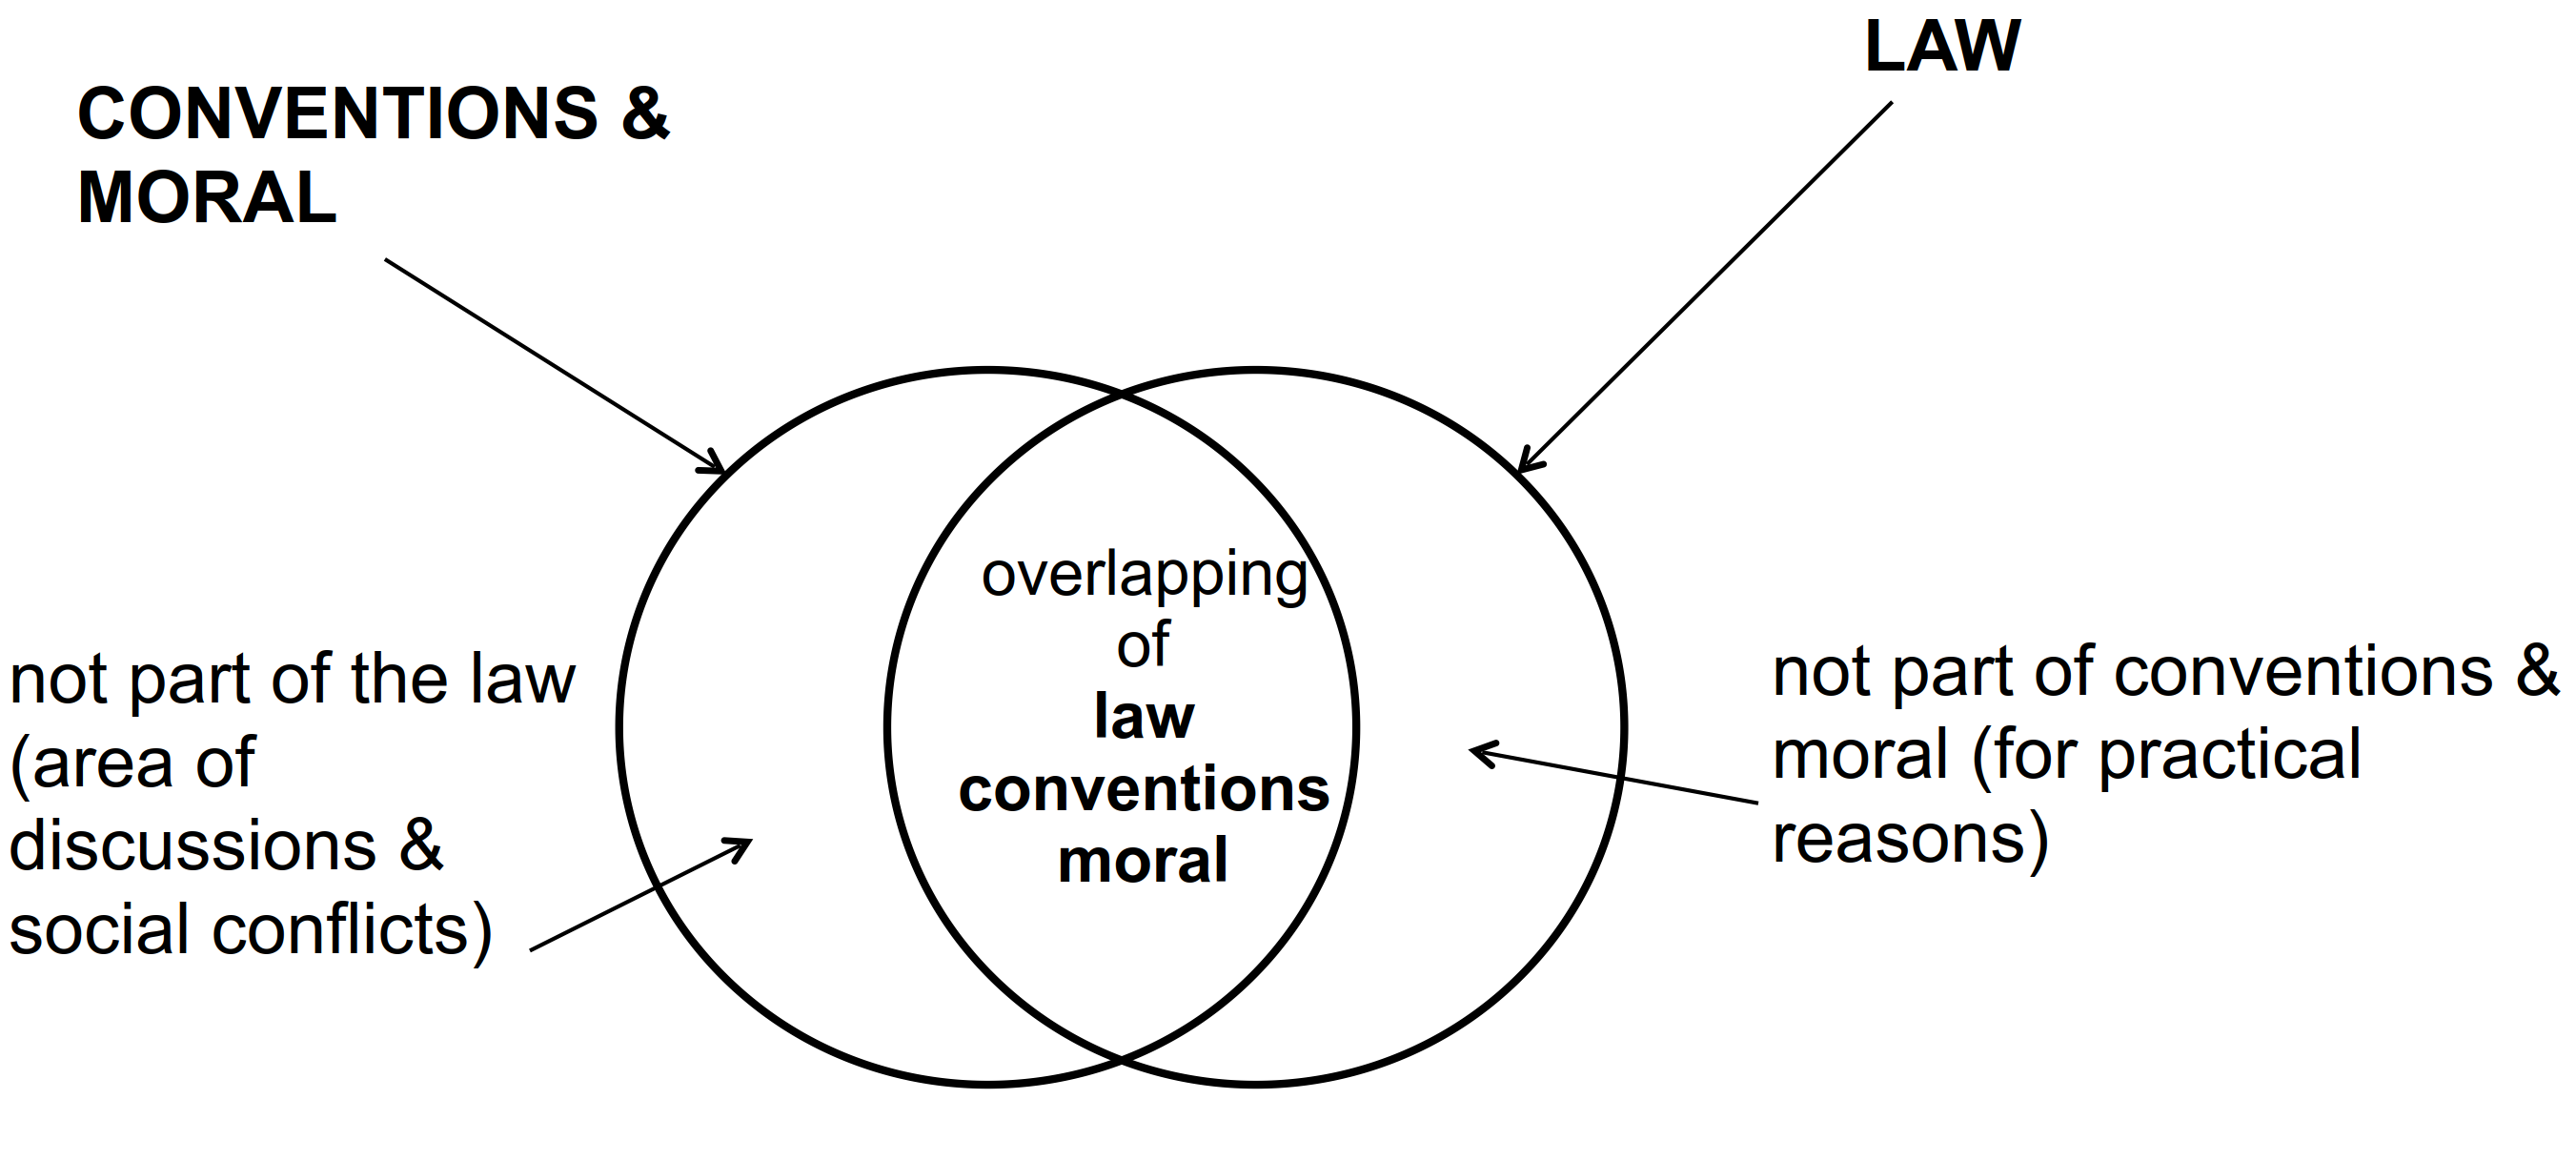
\includegraphics[width=1\linewidth]{images/conventions_moral_and_law}

\subsection{Law under different perspectives}
Classification is based upon:
\begin{compactitem}
	\item status (constitution, act, regulations/by-law)
	\item issuer (federal-, cantonal- and communal law)
	\item source of law (written law, common law, judicial tradition)
	\item involved person (civil law or public law)
\end{compactitem}

\subsection{Separation of Powers}
\begin{compactitem}
	\item „Das Schweizervolk und die Kantone bilden die Schweizerische Eidgenossenschaft“ (Art. 1 BV) – not vice-versa!
	\item „Der Kanton arbeitet mit den Gemeinden, den anderen Kantonen, dem Bund und, in seinem Zuständigkeitsbereich, mit dem Ausland zusammen.“ (§ 4 Kantonsverfassung ZH)
	\item The State is only entitled to legislate and to act in a territory/legal field if he has a constitutional legitimation!
	\item Cantons are in their power of legislation superior to the State!
\end{compactitem}

\subsection{Civil and Public Law}
\begin{compactitem}
	\item Civil law is mastered by the principle of freedom of coalition and freedom of contract.
	\item Public law is mastered by the principle of legality (control of power).
	\item This results into completely different jurisdiction (civil-/criminal-	or administrative court) with each different procedures and rights.
\end{compactitem}

\subsection{by-law (Verordnung) and order (Verfügung)}
\begin{compactitem}
	\item By-Law is a general, abstract regulation as part of a law.
	\item An Order is an individual, concrete application of law to a person (i.e. monetary fine for parking too long or a
	building permit).
\end{compactitem}

\subsection{Switzerland and foreign countries}
\begin{compactitem}
	\item We're integrated into a longtime European legal tradition and uni-/bilateral conventions.
	\item We have a long history in commercial relationship with other countries.
	\item The IPRG (Gesetz über das internationale Privatrecht) is our „gateway“ between swiss and foreign law.
	\item IPRG rules, which law (swiss or foreign) is applicable and which (swiss or foreign) court is competent.
	\item Parties can (in most cases) decide under which jurisdiction they want to handle their disputes and which court will be competent.
\end{compactitem}